\section{轮零件图制作}
在制作轮零件图之前,先将轮零件的三维模型另存在为“轮视图布局.dwg”,并以此副本来进行轮零件图的制作。
\subsection{制作图幅}
为方便控制视图位置,使轮零件的两个视图在图纸中分布比较均均美观,因此首先进行图幅的制作。
\begin{procedure}
\item 进行页面设置

首先点击“布局1”选项卡,从模型空间切换至图纸空间,参照第\ref{sec:lianjieganshitu}节中修改页面设置中的操作方法,将轮零件图的打印机绘图设备设置为“DWG TO PDF.pc3”,图纸幅面设置为“ISO A4(210.00x297.00毫米)”,打印方向设置为“横向”,并将打印机绘图设备特性中的“修改标准图纸尺寸(可打印区域)”设置为带装订边的图幅边尺寸。完成设置后的结果如图\ref{fig:lunshitu1} 所示。
\begin{lstlisting}
命令:pagesetup
\end{lstlisting}
\item 进行图层设置

新建“图框”图层,线型为“continuous”,线宽为0.5毫米;新建“尺寸标注”和“标题栏”图层,线型为“continuous”,线宽为默认;新建“中心线”图层,线型为“center",线宽为默认,结果如图\ref{fig:lunlayerset} 所示。
\begin{lstlisting}
命令:layer
\end{lstlisting}
\begin{figure}[htbp]
\centering
\begin{floatrow}[3]
\ffigbox{\caption{页面设置结果}\label{fig:lunshitu1}}{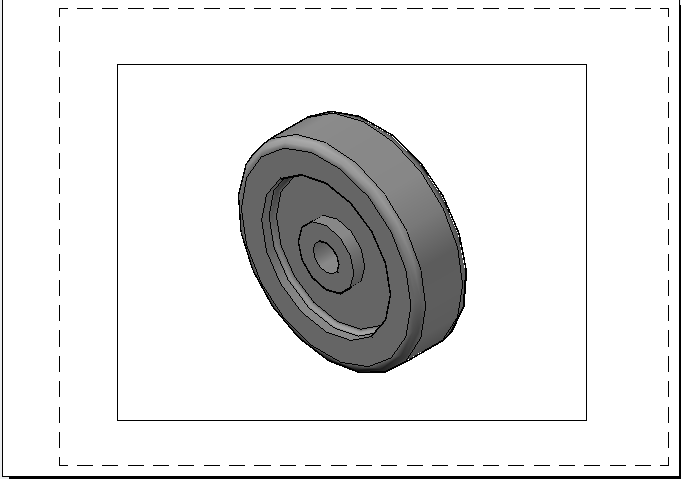
\includegraphics[scale=0.2]{lunshitu1}}
\ffigbox{\caption{新建图层结果}\label{fig:lunlayerset}}{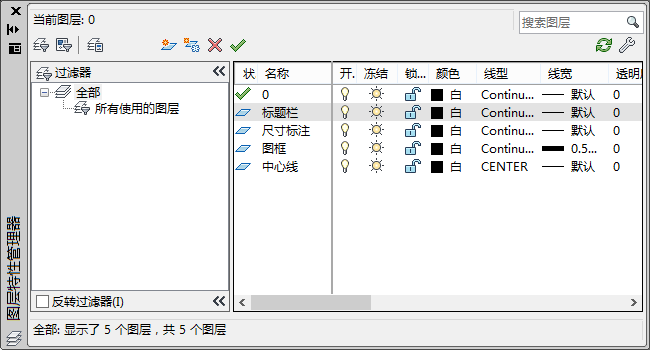
\includegraphics[scale=0.25]{lunlayerset}}
\ffigbox{\caption{图框绘制结果}\label{fig:lunshitu2}}{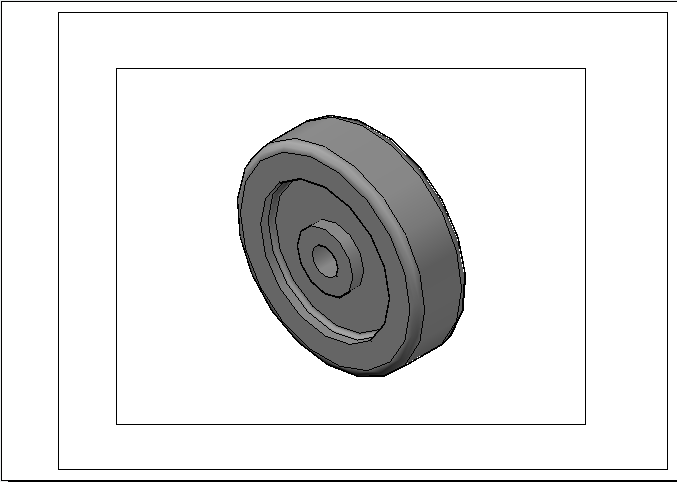
\includegraphics[scale=0.2]{lunshitu2}}
\end{floatrow}
\end{figure}
\item 绘制图框

将当前图层设置为“图框”图层,并绘制图框矩形,结果如图\ref{fig:lunshitu2} 所示。
\begin{lstlisting}
命令: RECTANG
指定第一个角点或 [倒角(C)/标高(E)/圆角(F)/厚度(T)/宽度(W)]: 0,0
指定另一个角点或 [面积(A)/尺寸(D)/旋转(R)]: 267,200
\end{lstlisting}

\item 插入标题栏

我们在\ref{sec:lianjieganshitu}节中制作了标题栏块并保为可以共享的文件,因此在本节中可以直接插入标题块来完成标题的制作。首先先将图层切换为“标题栏”图层,然后调用AutoCAD的块插入命令,其方法有:
\begin{itemize}
\item 键盘输入insert\index{insert,块插入}或I
\item 【插入】$\rightarrow $【块】
\item 【绘图】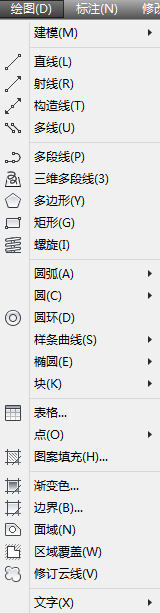
\includegraphics[scale=0.45]{drawtools} 工具栏中的
\includegraphics[scale=0.45]{blocktool}图标
\end{itemize}

\begin{figure}[htbp]
\centering
\subfloat[]{\label{fig:insertdialog}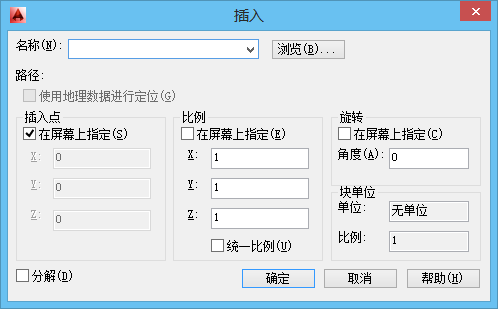
\includegraphics[scale=0.3]{insertdialog}}\hspace{20pt}
\subfloat[]{\label{fig:blockfileselect}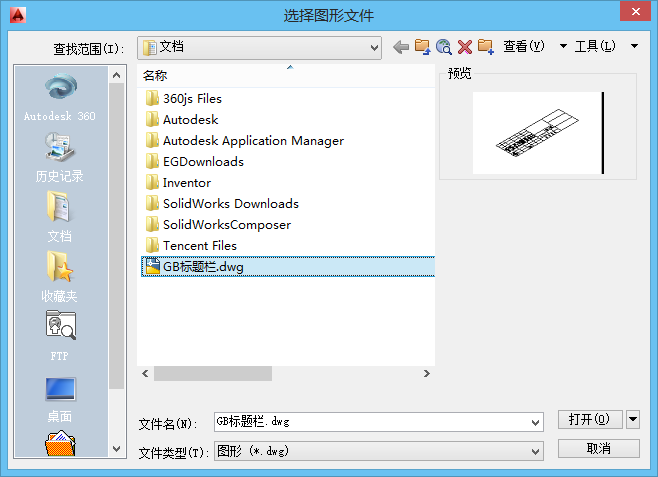
\includegraphics[scale=0.2]{blockfileselect.png}}\hspace{20pt}
\subfloat[]{\label{fig:insertdialog2}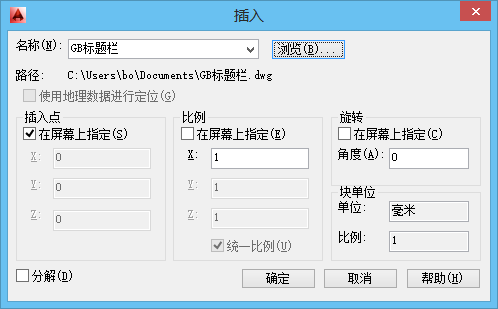
\includegraphics[scale=0.3]{insertdialog2.png}}
\caption{调入块文件过程}
\end{figure}

块插入命令启动后会弹出图\ref{fig:insertdialog}所示的插入对话框,由于标题栏块是以文件形式存在的,所以点击“名称”左边的浏览按钮,调出图\ref{fig:blockfileselect}所示的选择图形文件对话框,选择标题栏块文件所在的位置并选择,点击打开即完成标题块的载入,结果如图\ref{fig:insertdialog2}所示。

标题栏块加载后,点击确定按钮,命令会提示指定插入点,此时按图\ref{fig:insertbiaotilan} 所示位置选择块的插入点,完成后结果如图\ref{fig:lunshitu3} 所示。
\begin{lstlisting}
命令: INSERT
指定插入点或 [基点(B)/比例(S)/旋转(R)]:
\end{lstlisting}

\begin{figure}[htbp]
\centering
\subfloat[]{\label{fig:insertbiaotilan}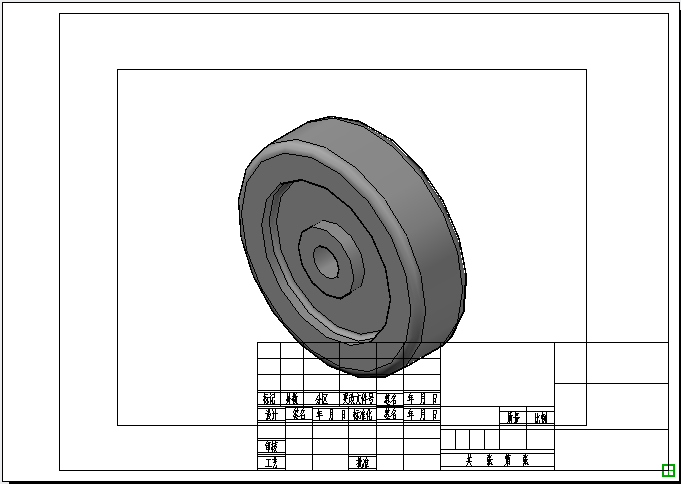
\includegraphics[scale=0.3]{insertbiaotilan}}\hspace{20pt}
\subfloat[]{\label{fig:lunshitu3}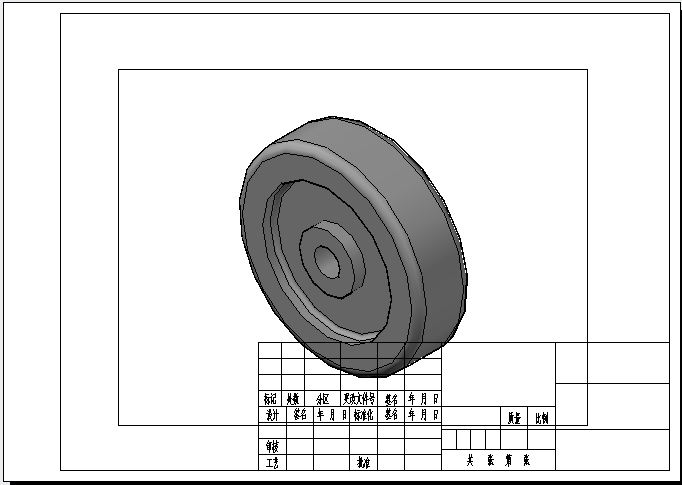
\includegraphics[scale=0.3]{lunshitu3}}
\caption{块插入过程}
\end{figure}
\end{procedure}
\subsection{制作视图}
\begin{procedure}
\item 删除当前视口

观察图\ref{fig:lunshitu3}可以看出,插入标题栏的标题与自动生成的视口存在交叉重叠,生成视图后会相互影响。由于标题栏的尺寸是国家校准规定的,是不能够更改的,所需要删除或修改自动生成的视口,以消除交叉重叠的情况。AutoCAD中调用删除命令的方法有:
\begin{itemize}
\item 键盘输入ERASE\index{erase,删除}或delete\index{delete,删除}或E
\item 【修改】$\rightarrow $【删除】
\item 【修改】
\includegraphics[scale=0.45]{edittools} 工具栏中的
\includegraphics[scale=0.45]{erase}图标
\end{itemize}

删除命令调用后用鼠标选择视口,选择完成后视口会以虚线的形式显示,如图\ref{fig:eraseselect}。删除后的结果如图\ref{fig:eraseresult}所示。

\begin{figure}[htbp]
\centering
\subfloat[]{\label{fig:eraseselect}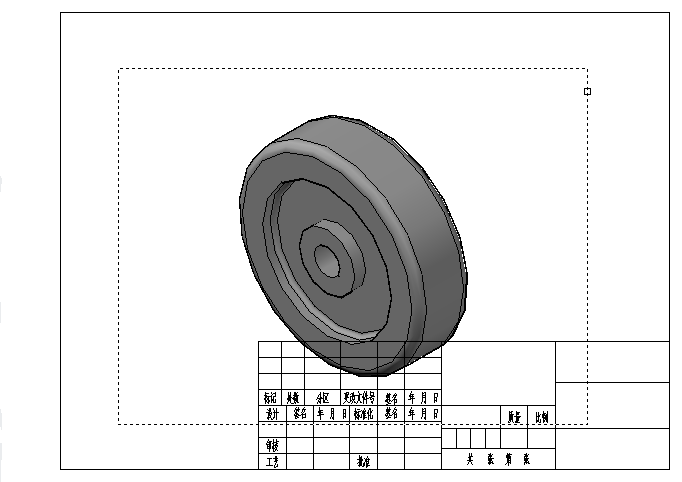
\includegraphics[scale=0.3]{eraseselect}}\hspace{20pt}
\subfloat[]{\label{fig:eraseresult}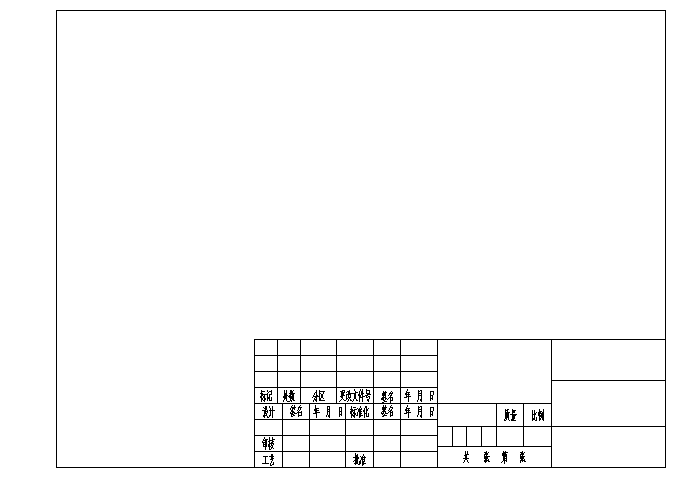
\includegraphics[scale=0.3]{eraseresult}}
\caption{删除视口过程}
\end{figure}
\begin{lstlisting}
命令: ERASE
选择对象: 找到 1 个
选择对象:
\end{lstlisting}

\item 新建视口

由于视口被删除后,图纸空间中已经没有轮零件的模型显示,因此需要在左视图位置新建一个视口来显示轮零件的左视图。AutoCAD中新建视口命令的调用方法有:
\begin{itemize}
\item 键盘输入-vports\index{-vports,新建视口}
\item 【视图】$\rightarrow $【视口】$\rightarrow $【一个视口】
\item 【视口】
\includegraphics[scale=0.45]{vportstools}工具栏中的【单个视口】
\includegraphics[scale=0.45]{vportssingle}图标
\end{itemize}

新建视口命令调用后提示指定视口的角点,此时按图\ref{fig:vportsfirstnode} 所示位置指定角点。

\begin{figure}[htbp]
\centering
\subfloat[]{\label{fig:vportsfirstnode}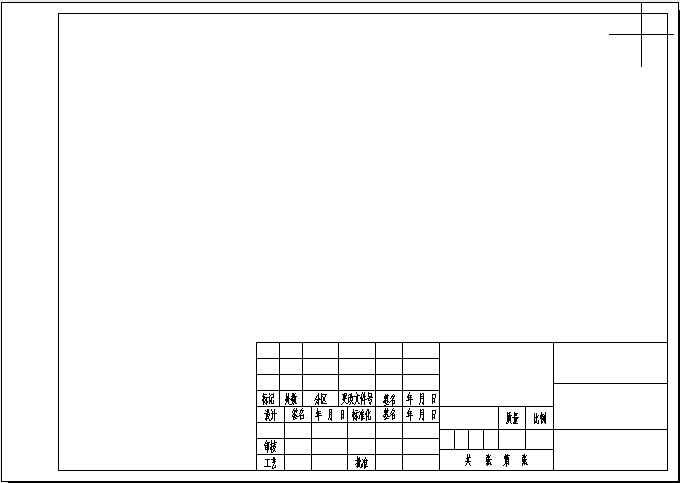
\includegraphics[scale=0.2]{vportsfirstnode}}\hspace{20pt}
\subfloat[]{\label{fig:vportssecondnode}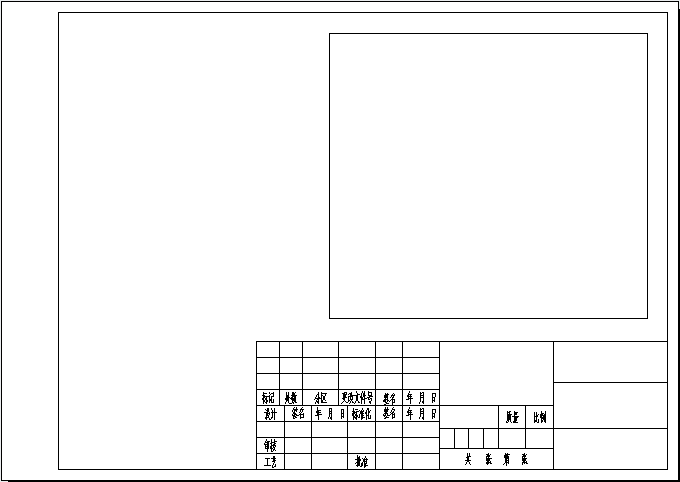
\includegraphics[scale=0.2]{vportssecondnode}}\hspace{20pt}
\subfloat[]{\label{fig:vportsresult}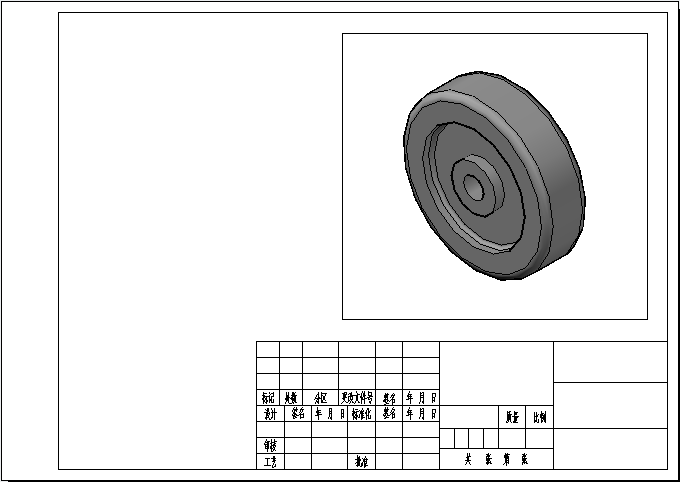
\includegraphics[scale=0.2]{vportsresult}}
\caption{新建视口过程}
\end{figure}
\begin{lstlisting}
命令: -VPORTS
指定视口的角点或 [开(ON)/关(OFF)/布满(F)/着色打印(S)/锁定(L)/对象(O)/多边形(P)/恢复(R)/图层(LA)/2/3/4] <布满>:
\end{lstlisting}

接下来,按图\ref{fig:vportssecondnode}所示位置指定对角点,完成后结果如图\ref{fig:vportsresult}所示。
\begin{lstlisting}
指定对角点:
\end{lstlisting}

\item 设置左视图

左视图视口建立完成后,通过双击或输入mspace命令进入视口模型空间。
\begin{lstlisting}
命令: MSPACE
\end{lstlisting}

接下来,将视图方向设置为左视图方向,并将视口比例设置为1:1。
\begin{lstlisting}
命令: -VIEW
输入选项 [?/删除(D)/正交(O)/恢复(R)/保存(S)/设置(E)/窗口(W)]: left
\end{lstlisting}

接下来,提取左视图轮廓,即完成左视图的生成。
\begin{lstlisting}
命令: solprof
选择对象: 找到 1 个
选择对象:
是否在单独的图层中显示隐藏的轮廓线?[是(Y)/否(N)] <是>:
是否将轮廓线投影到平面?[是(Y)/否(N)] <是>:
是否删除相切的边? [是(Y)/否(N)] <是>:
\end{lstlisting}

\item 生成全剖主视图

图\ref{fig:xiaolunlun.pdf}所示的轮零件图的主视图被称为全剖视图。剖视图是为克服由于物体内部形状较复杂时,视图虚线过多,读图和标尺寸困难的不足,而采取的有利于清晰表达物体内部形状的视图表达方法,它是假想用剖切面剖开物体,将位于观察者和剖切面之物的部分移去,而将其余部分向投影面投影所得的图形。所谓全剖视图是用剖切面将物体完全剖开后所得的剖视图。全剖视图适合表达内部开头比较复杂的物体。
\begin{enumerate}
\item 生成截面视图

在AutoCAD中,生成全剖主视图需要用到图纸视图命令,其调用方法有:
\begin{itemize}
\item 键盘输入solview\index{solview,图纸视图}
\item 【绘图】$\rightarrow $【建模】$\rightarrow $【设置】$\rightarrow $【视图】
\end{itemize}

图纸视图命令调用后,提示输入选项,由于要生成全部剖视图,需要指定其假想的剖切面,因此选择【截面(s)】选项。
\begin{lstlisting}
命令: solview
输入选项 [UCS(U)/正交(O)/辅助(A)/截面(S)]: s
\end{lstlisting}

接下来命令提示指定剪切平面的第一个点,此时按图\ref{fig:solviewfirstnode}所示的对象捕捉追踪方式设置第一个点。

\begin{figure}[htbp]
\centering
\subfloat[]{\label{fig:solviewfirstnode}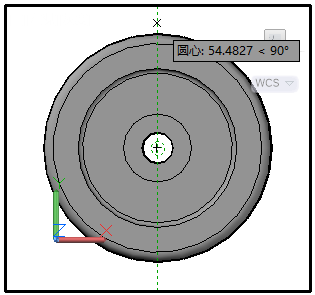
\includegraphics[scale=0.4]{solviewfirstnode}}\hspace{20pt}
\subfloat[]{\label{fig:solviewsecondnode}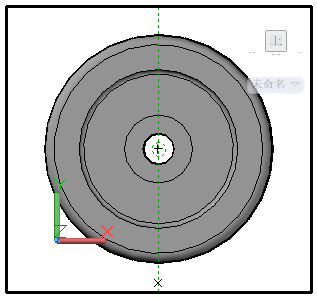
\includegraphics[scale=0.4]{solviewsecondnode}}\hspace{20pt}
\subfloat[]{\label{fig:solview1}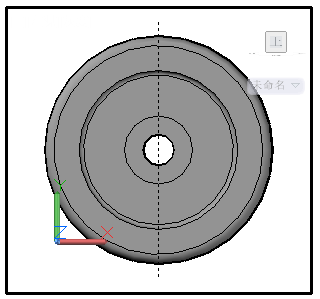
\includegraphics[scale=0.4]{solview1}}
\caption{截面视图生成过程(一)}
\end{figure}

\begin{lstlisting}
指定剪切平面的第一个点:
\end{lstlisting}

接下来,以图\ref{fig:solviewsecondnode}所示的方式指定剪切平面的第二个点,完成后的效果如图\ref{fig:solview1}所示。
\begin{lstlisting}
指定剪切平面的第二个点:
\end{lstlisting}

由于主视图位于左视视的左边,因此需要从左视图的右边向左边观察,因此用鼠标点击图\ref{fig:solview1}中虚线的右侧,以指定观察侧。
\begin{lstlisting}
指定要从哪侧查看:
\end{lstlisting}

接下来,指定视图比例,一般情况下都是直接确认默认值。
\begin{lstlisting}
输入视图比例 <1>:
\end{lstlisting}

接下来以图\ref{fig:solview2}所示的位置作为视图的中心。
\begin{lstlisting}
指定视图中心:
指定视图中心 <指定视口>:
\end{lstlisting}

\begin{figure}[htbp]
\centering
\subfloat[]{\label{fig:solview2}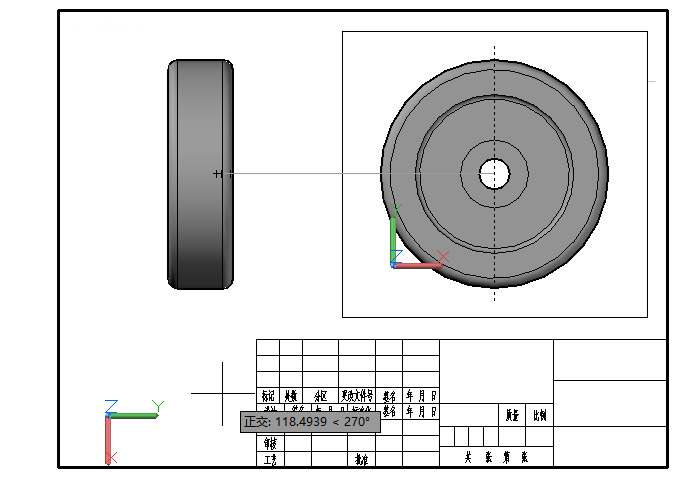
\includegraphics[scale=0.3]{solview2}}\hspace{20pt}
\subfloat[]{\label{fig:solview3}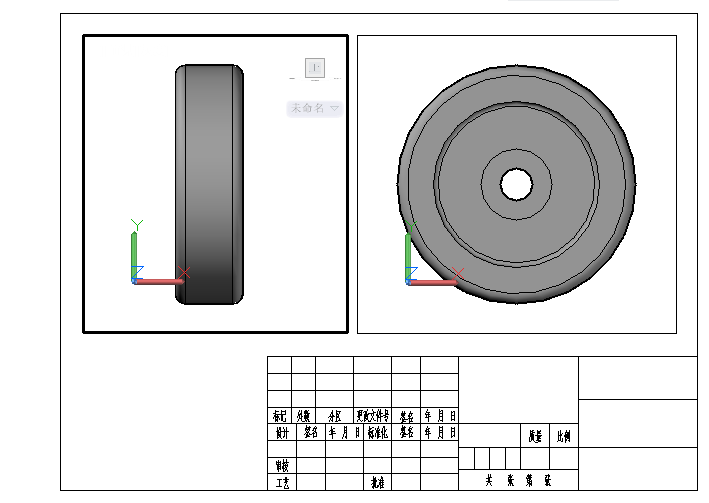
\includegraphics[scale=0.3]{solview3}}
\caption{截面视图生成过程(二)}
\end{figure}

接下来以用鼠标确主视图视口的两个角点。
\begin{lstlisting}
指定视口的第一个角点:
指定视口的对角点:
\end{lstlisting}

指定“F”作为视图名称即可完成截面视图的生成,其效果如图\ref{fig:solview3} 所示。
\begin{lstlisting}
输入视图名: f
输入选项 [UCS(U)/正交(O)/辅助(A)/截面(S)]:
\end{lstlisting}

\item 图形化截面视图

截面视图生成后,还需要将其图形化后,才能够真正地生成剖视图。AutoCAD中调用视图图形化命令的方式有:
\begin{itemize}
\item 键盘输入soldraw\index{soldraw,视图图形化}
\item 【绘图】$\rightarrow $【建模】$\rightarrow $【设置】$\rightarrow $【图形】
\end{itemize}

调用图形化命令后选择主视图所在的视口作为要绘图的视口,选择后的效果如图
\begin{lstlisting}
命令: soldraw
选择要绘图的视口...
选择对象: 找到 1 个
选择对象:
\end{lstlisting}

\begin{figure}[htbp]
\centering
\subfloat[]{\label{fig:soldraw1}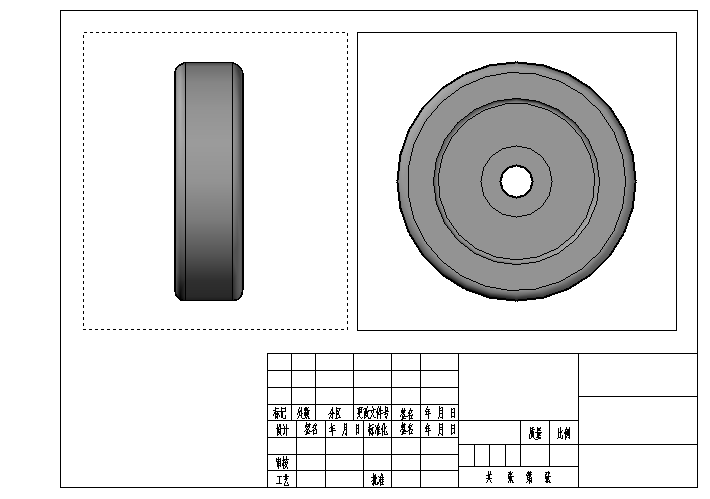
\includegraphics[scale=0.3]{soldraw1}}\hspace{20pt}
\subfloat[]{\label{fig:soldraw2}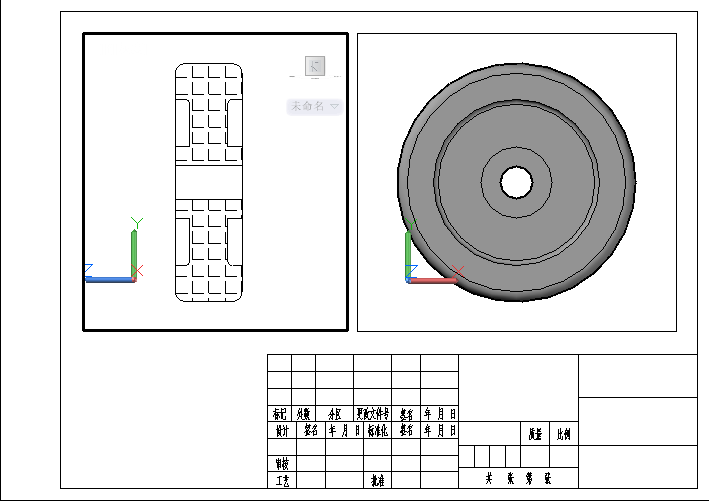
\includegraphics[scale=0.3]{soldraw2}}
\caption{图形化操作}
\end{figure}

\item 修改填充图案

通常情况下,图化后的填充图案并不符合国家标准的要求,需要进行修改。AutoCAD中修改填充图案需要调用编辑填充图案命令,其方式有:
\begin{itemize}
\item 键盘输入hatchedit\index{hatchedit,编辑图案填充}
\item 【修改】$\rightarrow $【对象】$\rightarrow $【图案填空】
\item 【修改II】
\includegraphics[scale=0.45]{modifyIItools}工具栏中的【编辑图案填充】
\includegraphics[scale=0.45]{hatchedidtool}图标
\end{itemize}

编辑填充图案命令调用后,提示选择图案填充对象。选择主视图中的填充图案后会弹出图\ref{fig:hatcheditdialog}所示的图案填充编辑对话框,点击样例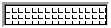
\includegraphics[scale=0.4]{hatchpicture}图案,弹出图\ref{fig:hatchfillpicture}所示的填充图案选项板,然后点选ANSI选项卡,如图\ref{fig:hatchfillselect}所示。选择ANSI37图案并确定,修改后的结果如图\ref{fig:lunshitu5}所示。
\begin{lstlisting}
命令: hatchedit
选择图案填充对象:
\end{lstlisting}

\begin{figure}[htbp]
\centering
\subfloat[]{\label{fig:hatcheditdialog}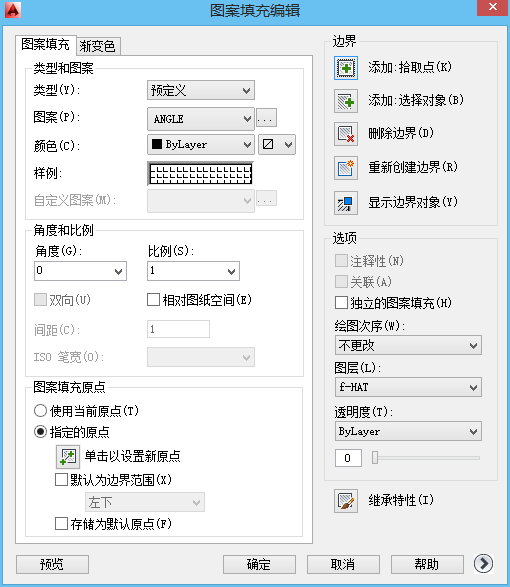
\includegraphics[scale=0.25]{hatcheditdialog}}\hspace{20pt}
\subfloat[]{\label{fig:hatchfillpicture}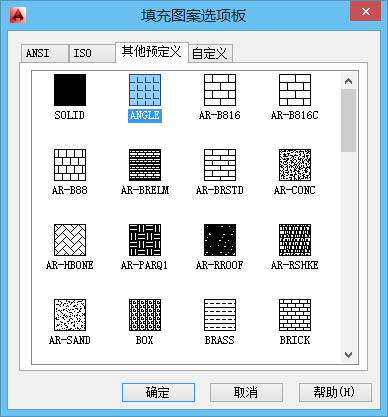
\includegraphics[scale=0.35]{hatchfillpicture}}\\
\subfloat[]{\label{fig:hatchfillselect}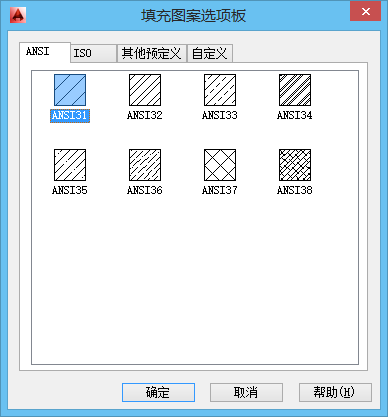
\includegraphics[scale=0.35]{hatchfillselect}}\hspace{20pt}
\subfloat[]{\label{fig:lunshitu5}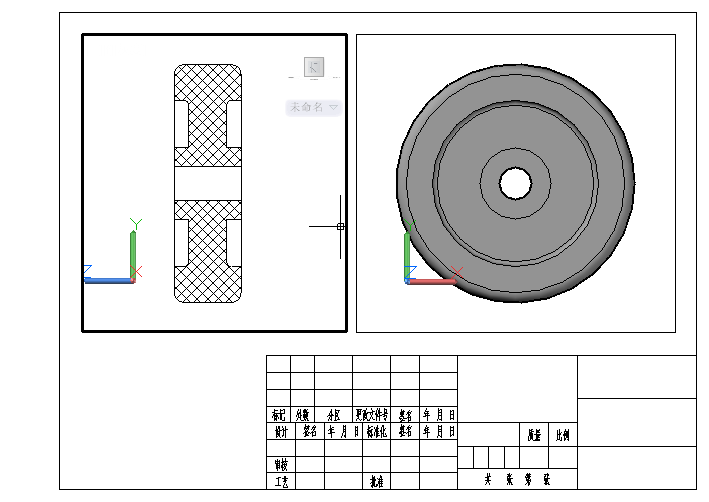
\includegraphics[scale=0.3]{lunshitu5}}
\caption{修改图案填充}
\end{figure}

\end{enumerate}
\item 调整图层设置

首先退出模型空间,防止错误的鼠标缩放操作改变视口的显示比例,导致对应关系错误。

\begin{lstlisting}
命令: PSPACE
\end{lstlisting}

按图 所示结果设置图层,设置完成后的轮零件图效果如图 所示。
\begin{lstlisting}
命令:layer
\end{lstlisting}

\begin{figure}[htbp]
\centering
\begin{floatrow}[2]
\ffigbox{\caption{图层设置结果}\label{fig:lunshitulayer}}{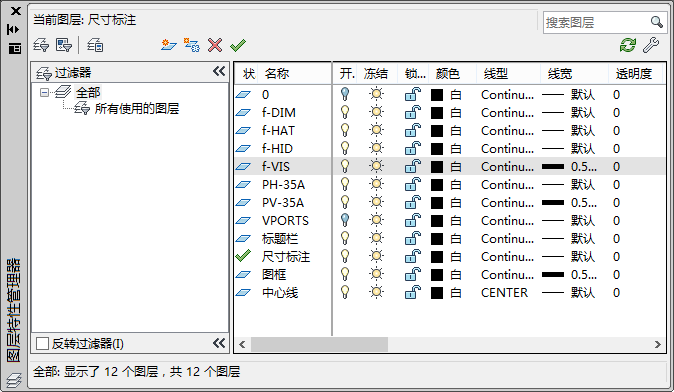
\includegraphics[scale=0.3]{lunshitulayer}}
\ffigbox{\label{fig:lunshituresult1}}{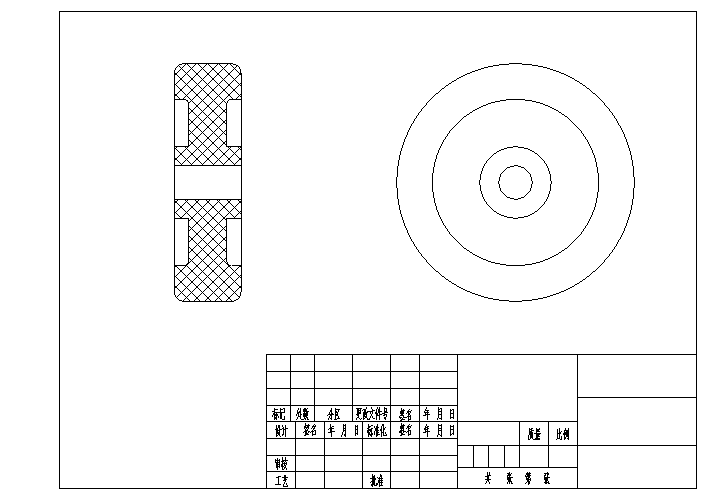
\includegraphics[scale=0.3]{lunshituresult1}}
\end{floatrow}
\end{figure}

\end{procedure}
\subsection{标注尺寸}

\begin{figure}[htbp]
\centering
\subfloat[]{\label{fig:lunshitu6}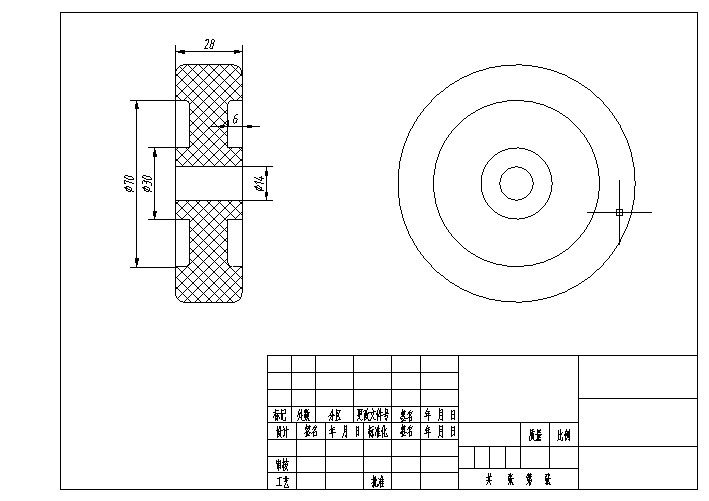
\includegraphics[scale=0.3]{lunshitu6}}\hspace{20pt}
\subfloat[]{\label{fig:lunshitu7}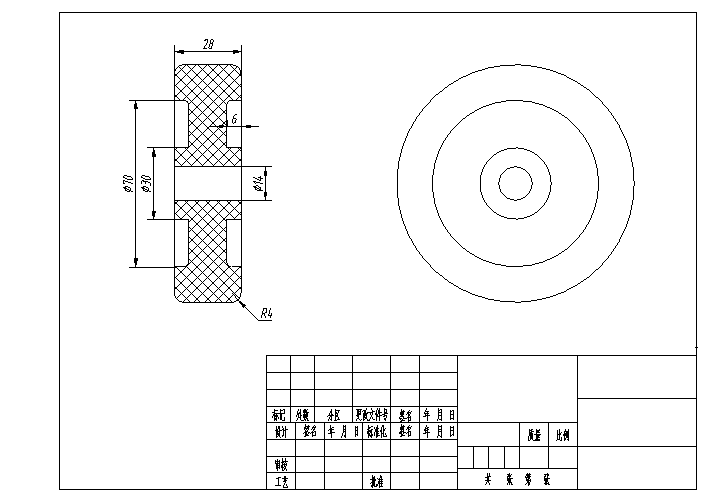
\includegraphics[scale=0.3]{lunshitu7}}\\
\subfloat[]{\label{fig:lunshitu8}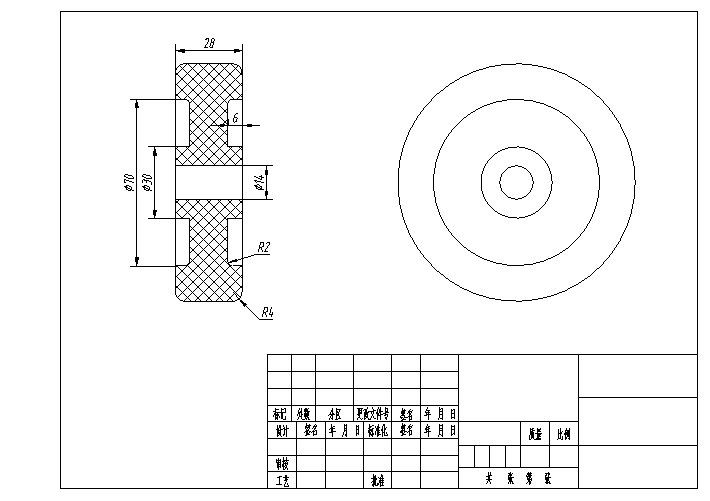
\includegraphics[scale=0.3]{lunshitu8}}\hspace{20pt}
\subfloat[]{\label{fig:lunshitu9}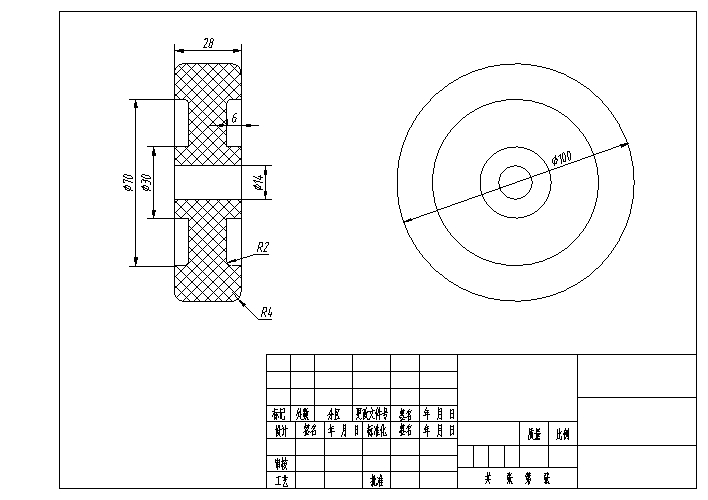
\includegraphics[scale=0.3]{lunshitu9}}
\caption{尺寸标注}

\end{figure}
\begin{procedure}
\item 设置标注样式

按\ref{sec:lianjieganshitu}节的步骤设置标注样式。

\item 标注线性尺寸

按\ref{sec:lianjieganshitu}节的步骤进行线性尺寸的标注,结果如图\ref{fig:lunshitu6} 所示。


\item 标注半径尺寸

圆弧的尺寸必须要使用半径方式进行标注。AutoCAD中标注半径需要调用半径标注命令,其调用方法有:
\begin{itemize}
\item 键盘输入dimradius\index{dimradius,半径标注}
\item 【标注】$\rightarrow $【半径】
\item 【标注】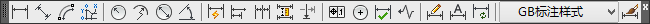
\includegraphics[scale=0.45]{dimtoolsbar}工具栏中的【半径】
\includegraphics[scale=0.45]{dimradius}图标
\end{itemize}

半径标注命令调用后,选择主视图右下角的$R4$圆弧进行标注,结果如图\ref{fig:lunshitu7}所示。
\begin{lstlisting}
命令: dimradius
选择圆弧或圆:
标注文字 = 4
指定尺寸线位置或 [多行文字(M)/文字(T)/角度(A)]:
\end{lstlisting}

以相同的方式完成$R2$圆弧的标注,结果如图\ref{fig:lunshitu8}所示。
\item 标注直径尺寸

圆的标注必须使用直径的方式进行标注,AutoCAD中直径标注命令的调用方式有:
\begin{itemize}
\item 键盘输入dimdiameter\index{dimdiameter,直径标注}
\item 【标注】$\rightarrow $【直径】
\item 【标注】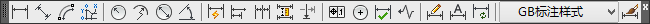
\includegraphics[scale=0.45]{dimtoolsbar}工具栏中的【半径】
\includegraphics[scale=0.45]{dimdiameter}图标
\end{itemize}

直径标注命令调用后,选择左视图中最大的圆作为标注对象,结果如图\ref{fig:lunshitu9}所示。

\begin{lstlisting}
命令: dimdiameter
选择圆弧或圆:
标注文字 = 100
指定尺寸线位置或 [多行文字(M)/文字(T)/角度(A)]:
\end{lstlisting}
\end{procedure}
\endinput